\chapter{Development of Hybrid Targets}
\label{chap4}

\section{Overview}

In this chapter, I present the development of high-performance polarized $^{3}$He targets for use in electron scattering experiments that utilize the technique of alkali-hybrid spin-exchange optical pumping~\cite{PhysRevC.91.055205}. Data from 24 separate target cells are presented, each of these cells was constructed while preparing for one of four experiments at Jefferson Laboratory (JLAB). The results document dramatic improvement in the performance of polarized $^{3}$He targets. I focus on the data analysis work in this chapter since most of the data had already been taken by the time I joined the group. Other details are described by Jaideep Singh~\cite{PhysRevC.91.055205}. With the wide range of data, we successfully determined the so-called X-factors that quantify an as-yet poorly understood spin-relaxation mechanism that limits the maximum achievable $^{3}$He polarization to well under 100\%. The data collected also served as a measurement of the K-$^{3}$He spin-exchange rate coefficient $k_{se}^{K}=(7.46\pm0.62)\times10^{-20}$ cm$^{3}$/s over the temperature range 503 K to 563 K.

\section{Development of Hybrid Targets}

Spin-exchange optical pumping (SEOP) is a two step process in which an alkali-metal vapor is polarized with optical pumping which subsequently polarizes noble-gas nuclei via spin-exchange collisions\cite{WalkerHapper}. A pure Rb vapor was used to polarize $^{3}$He prior to the development of hybrid cells. However, it was found that K is far more efficient than Rb at transferring its polarization to $^{3}$He nuclei~\cite{PhysRevLett.80.2801}. Hybrid mixtures of Rb and K have subsequently been used to improve the efficiency of the polarization process~\cite{PhysRevA.75.013416, PhysRevA.56.2090, PhysRevLett.80.2801}. In alkali-hybrid spin-exchange optical pumping (AHSEOP), the Rb vapor is polarized by circularly polarized laser light, but the polarization of Rb valence electrons is then rapidly shared with the K~\cite{PhysRevLett.91.123003}. The rate at which Rb and K exchange polarization is so fast, for our purposes here, that their polarizations can be thought of as being equal. If the alkali-hybrid mixture contains significantly more K than Rb with an appropriate ratio, the spin-exchange efficiency is greatly improved so that the rate at which $^{3}$He is polarized is increased significantly for a given amount of laser power.

The second factor that proved to have improved target cells performance greatly was the use of spectrally-narrowed diode lasers~\cite{JAP.94.6908}. We were able to achieve higher alkali polarization with the aid of these lasers, which in turn reduced the required laser power. The origins of the improved cell performance are twofold. Firstly, these narrowband lasers have spectral profiles more closely matched to the Rb D$_{1}$ absorption line shapes, which results in higher optical pumping rates and hence higher alkali polarizations. Secondly, they contribute to allowing us to use higher alkali densities (which increases spin-exchange rates) without sacrificing alkali polarization. 

The data collected over the years include $^{3}$He polarization achieved under different operating conditions, the time constants of polarization process, the geometric properties of the target cells, and cell fill information such as pressure and ratio of K to Rb in hybrid mixtures and the time constants of the spin-relaxation process. In roughly half the cells, the alkali polarization and alkali density were also measured with Faraday rotation techniques. The results contain several thousand hours worth of data and provide valuable information for future cell development.

Two figures of merit (FOMs) are plotted in Fig.~\ref{fig:foms}, both of which are relevant in evaluating the performance of a polarized $^{3}$He target. The one on the left axis is the effective luminosity $\mathcal{L}^{eff}=\mathcal{L}P_{He}^{2}$, where $\mathcal{L}$ is the luminosity for a fixed-target experiment (the product of beam current, target density, and interaction length) and $P_{He}$ is the $^{3}$He polarization. The luminosity $\mathcal{L}$ represents the number of scattering opportunities per unit time per unit area, while $P_{He}^{2}$ accounts for the reduction in effective statistics when measuring a polarization-dependant asymmetry. The FOM on the right axis is used to quantify the potential effective luminosity of a target. The definition is $\mathcal{L}^{N}=\mathcal{N}\Gamma_{s}P_{He}^{2}$, where $\mathcal{N}$ is the total number of $^{3}$He atoms in the target and $\Gamma_{s}$ is the rate at which polarization builds up. The target cell Antoinette was the first one with such a high value of $\mathcal{L}^{N}$, which indicated the cell could tolerate higher luminosities than previously achieved. The high potential further demonstrates the importance of the development of the new convection style target cell~\cite{PhysRevC.84.065201}. With even higher luminosities in electron scattering experiments, significantly faster gas transfer becomes quite necessary to reduce the ``polarization gradient" between the pumping chamber of target chamber.

\begin{figure}[t!]
	\centering
	\resizebox{0.91\textwidth}{!}{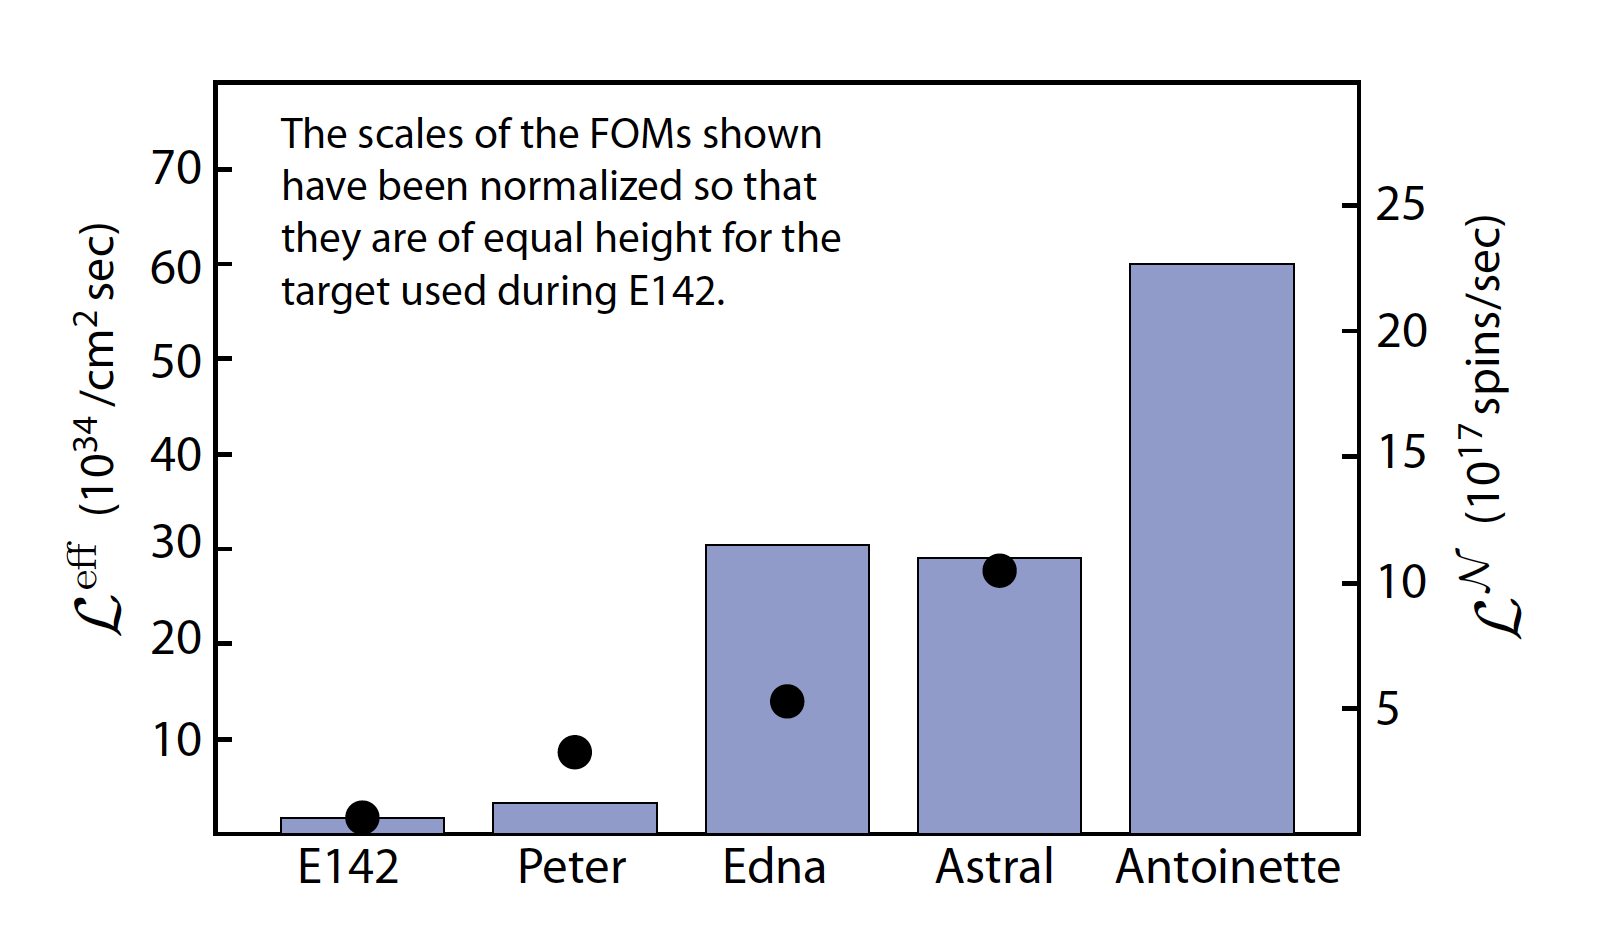
\includegraphics{target_performance.png}}
	\caption{{Shown are two figures of merit (FOM) for targets built for the indicated experiments.  The circles (left axis) indicate the luminosity weighted by the square of polarization.  The bars (right axis) represent the total number of spins being polarized per second weighted by the square of polarization.  While the right FOM is an indication of the potential of the polarization technique, the left FOM indicates performance achieved during an experiment. The scales have been normalized so that the two FOMs have the same height for the cell marked E142}}
	\label{fig:foms}
\end{figure}

\subsection{Experimental Methods}

\subsubsection{The $^{3}$He Targets}

Chapter 2 has already described single-chambered cell polarization dynamics to some extent as it is a simpler model for introducing spin-exchange optical pumping. The $^{3}$He target cells JLab uses for electron scattering experiments usually include two chambers, a pumping chamber (PC), which is placed in an oven and pumped by circularly polarized laser light, and a target chamber (TC) that the electron beam passes through. Fig.\ref{TargetCell} shows a schematic representation of a typical cell. 

\begin{figure}[H]
	\centering
	\resizebox{0.91\textwidth}{!}{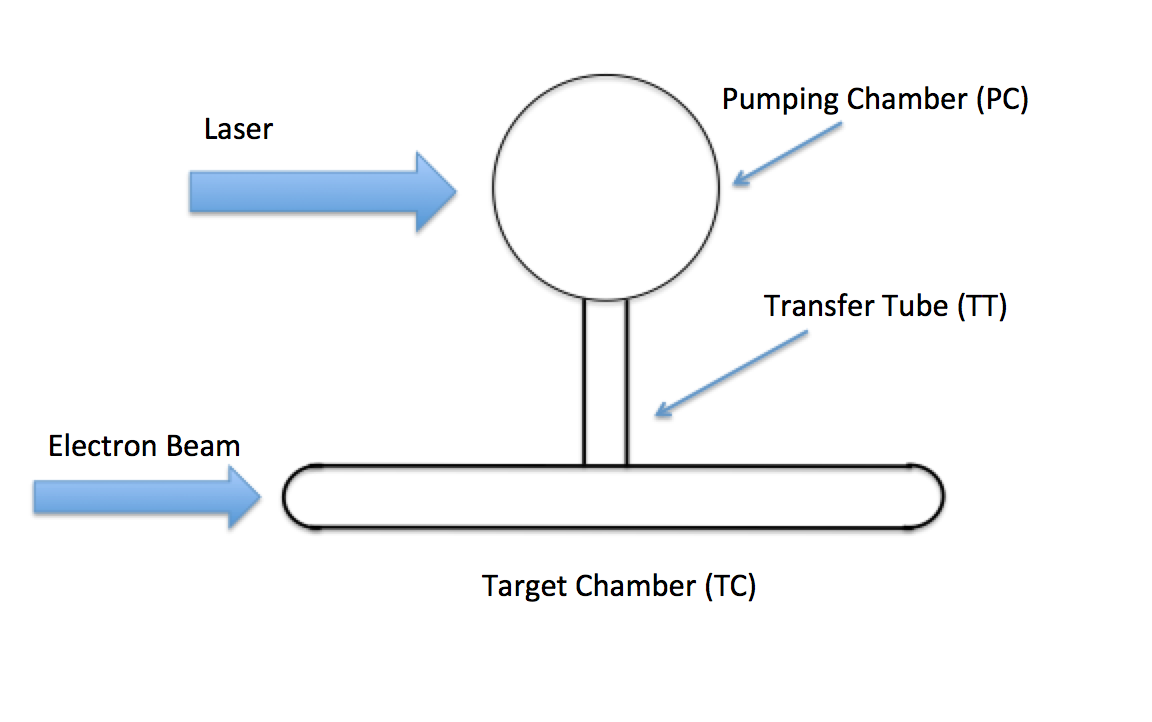
\includegraphics{TargetCell.png}}
	\caption{{ A target cell. The dimensions of different parts of the cell are not to scale.}}
	\label{TargetCell}
\end{figure}

After baking the cell to remove moisture and other contaminants, mixtures of Rb and K are ``chased" into the cell with a hand torch. Once the cell has been pumped with a diffusion pump for about a week, we can fill the cell with N$_{2}$ and $^{3}$He. 

The $^{3}$He density is of great importance for characterizing the target cells. One way to determine the $^{3}$He density is through measurements during the cell-filling process. A carefully calibrated volume, together with pressure and temperature measurements gives the volume of different spaces in the gas system (the system that is used to pump the cell and fill it with N$_{2}$ and $^{3}$He) and the cell itself. By comparing the amount of $^{3}$He left in the system, the amount that went into the cell is obtained. The volume of the cell can be measured by determining its buoyancy force in water. The $^{3}$He density is determined to within about 1\% with the method.

Another method that can be used for determining the $^{3}$He density is through measurements of the pressure broadening of the D$_{1}$ and D$_{2}$ absorption lines with a scannable single-frequency laser~\cite{Romalis1997}. This measurement also provides the value of D, which we defined as the ratio of K vapor density to Rb vapor density. Although the value of D is for the temperature at which the measurement is performed, its value for operating conditions can be inferred with alkali-metal vapor pressure curves. D can also be measured with the Faraday rotation technique in many cases, and the two methods agree with each other quite well. The fill densities and geometric properties of the aforementioned 24 cells are shown in Table~\ref{fill_densities}.

\begin{table*}\scriptsize 
	\begin{center}
		\begin{tabular}{|c|c|c|c|c|c|}
			\hline
			\multirow{2}{*}{\begin{sideways}{EXP}\end{sideways}}&\multirow{2}{*}{Cell} & Total & PC & \multirow{2}{*}Fill & TC   \\
			&& Volume(cc) & Volume(cc) & Density(amg) & length(cm)\\
			\hline
			\hline
			\multirow{5}{*}{\begin{sideways}saGDH\end{sideways}} 
			& Proteus & 235.9 & 90.8 & 6.88 & 34.3\\
			\cline{2-6}
			& Peter & 208.6 & 111.3 & 8.80 & 39.4\\
			\cline{2-6}
			& Penelope & 204.3 & 102.2 & 8.93 & 39.7\\
			\cline{2-6}
			& Powell & 213.3 & 111.6 & 8.95 & 40.5\\
			\cline{2-6}
			& Prasch & 257.7 & 114.5 & 6.94 & 35.3\\
			\hline
			\hline
			\multirow{9}{*}{\begin{sideways}GEN\end{sideways}} 
			& Al & 168.4 & 90.2 & 8.91 & 38.4\\ \cline{2-6}
			& Barbara & 386.2 & 306.8 & 7.60 & 38.7 \\ \cline{2-6}
			& Gloria & 378.2 & 298.8 & 7.40 & 38.4\\ \cline{2-6}
			& Anna & 386.8 & 303.7 & 8.09 & 38.7\\ \cline{2-6}
			& Dexter & 181.4 & 99.3 & 9.95 & 38.7\\ \cline{2-6}
			& Edna & 378.3 & 290.3 & 7.47 & 38.7\\ \cline{2-6}
			& Dolly & 378.3 & 293.5 & 7.42 & 38.7\\ \cline{2-6}
			& Simone & 219.5 & 118.6 & 8.17 & 37.9\\ \cline{2-6}
			& Sosa & 388.8 & 304.7 & 7.96 & 38.7\\ \hline
			\multirow{10}{*}{\begin{sideways}Transversity and $d_{2}^{n}$\end{sideways}} 
			& Boris & 246.1 & 166.1 & 8.08 & 38.4\\ \cline{2-6} 
			& Samantha & 259.0 & 176.9 & 7.97 & 38.4\\ \cline{2-6}
			& Alex & 278.3 & 193.9 & 7.73 & 39.1\\ \cline{2-6}
			& Moss & 269.8 & 184.7 & 7.92 & 38.7\\ \cline{2-6}
			& Tigger & 271.7 & 186.9 & 7.81 & 38.7\\ \cline{2-6}
			& Astral & 251.4 & 164.9 & 8.18 & 38.4\\ \cline{2-6}
			& Stephanie & 244.3 & 164.9 & 8.10 & 38.5\\ \cline{2-6}
			& Brady & 249.9 & 169.3 & 7.88 & 38.4\\ \cline{2-6}
			& Maureen & 268.5 & 177.4 & 7.63 & 39.8\\ \cline{2-6}
			& Antoinette & 437.8 & 351.8 & 6.57 & 40.3\\ \hline
		\end{tabular}
	\end{center}
	\caption{The table contains the names, total and pumping chamber volumes, fill densities and target chamber lengths of the 24 target cells. The fill densities are the average of the results from gas system measurements and pressure broadening measurements.}
	\label{fill_densities}
\end{table*}

\subsubsection{Target Cell Polarization Dynamics}

As previously mentioned, AFP is used to monitor the polarization of $^{3}$He~\cite{Abragam}. An absolute value of polarization remains to be calibrated with EPR, but the signal size is directly proportional to the polarization, thus is an indication of how the polarization changes relatively. Two processes that are monitored with AFP are spinups and spindowns. The details of the dynamics has been discussed in detail by Dolph \emph{et al.}~\cite{PhysRevC.84.065201}.

The study of the build up of $^3$He polarization by spin-exchange optical pumping is something referred to here as spinup. A typical example of a spinup is shown in Fig.~\ref{spinup}.

\begin{figure}[H]
	\centering
	\resizebox{0.91\textwidth}{!}{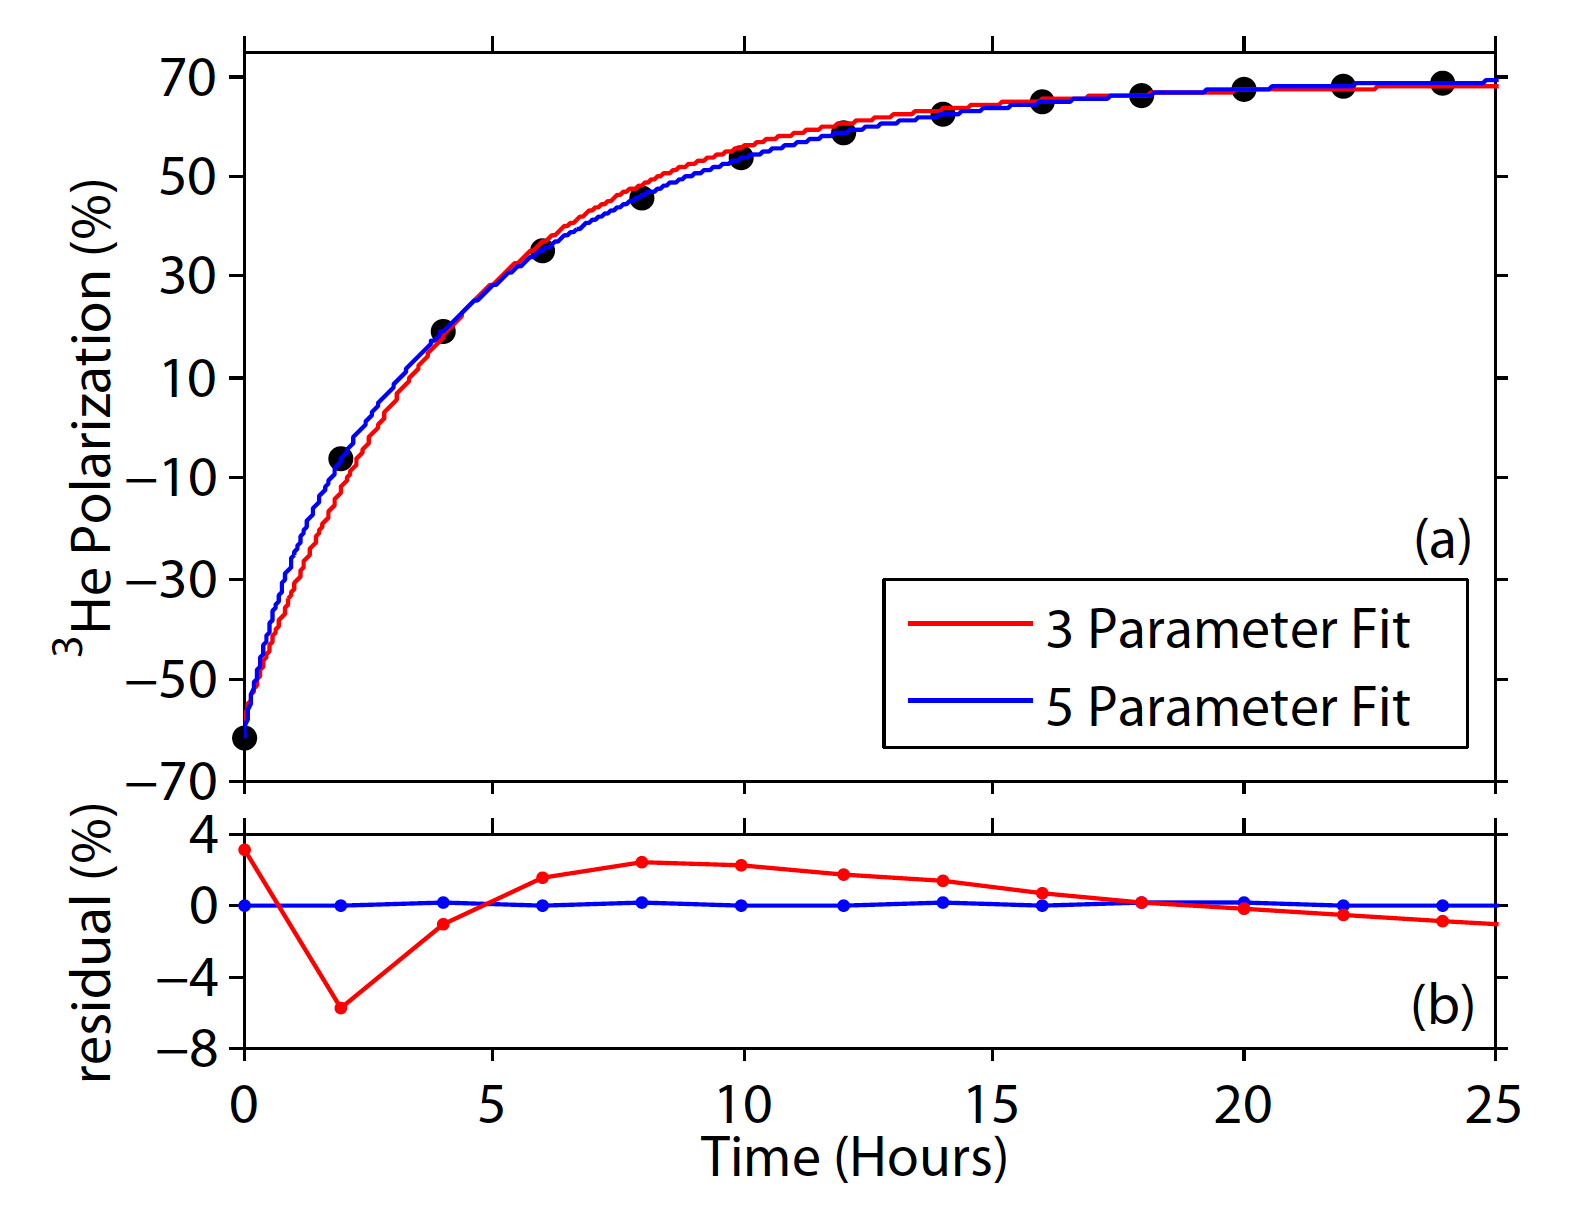
\includegraphics{Spinup.png}}
	\caption{{(a) Shown is a spinup of the target Brady. The spinup data has been fit with a 3-parameter and a 5-parameter formalism. (b) The residuals of the two fits. The error for 3-parameter fit is larger because it does not account for diffusion between two chambers.}}
	\label{spinup}
\end{figure}

The equation that describes spinups of a single-chambered cell is: 

\begin{equation}
P(t)=(P^{0}-P^{\infty})e^{-\Gamma_{sc}t}+P^{\infty}
\end{equation}
where $P^{\infty}$ is the saturation polarization, $P^{0}$ is the initial polarization, $\Gamma_{sc}=\gamma_{se}(1+X)+\Gamma$ is the spin-up rate of the buildup of polarization. The subscript ``sc" here stands for ``single chamber" to differ from the spinup rate of double-chambered cell. $\gamma_{se}$ is the spin-exchange rate, X is a parameter used to characterize a source of spin relaxation that limits the maximal achievable polarization, which will be discussed in more detail later in the chapter. $\Gamma$ is the spin relaxation rate due to mechanisms other than spin-exchange and that that is characterized by the parameter X. Often $\Gamma$ is dominated by relaxation at the cell walls. When using this equation to fit spinup, there are only three parameters, hence the name 3-parameter fit. The saturation polarization is given by:

\begin{equation}
P^{\infty}=\frac{\langle P_{A}\rangle \gamma_{se}}{\Gamma_{sc}}=\frac{\langle P_{A}\rangle\gamma_{se}}{\gamma_{se}(1+X)+\Gamma}
\end{equation}
where $\langle P_{A}\rangle$ is the polarization of the alkali vapor averaged over the cell.

The following derivation will only focus on double-chambered cell. The polarization accumulation rate can be described by 

\begin{subequations}\label{DoubleChamber}
	\begin{gather}
	\frac{dP_{pc}}{dt}=\Gamma_{se}(P_{A}-P_{pc})-\Gamma_{pc}P_{pc}-d_{pc}(P_{pc}-P_{tc})\\
	\frac{dP_{tc}}{dt}=-\Gamma_{tc}P_{tc}+d_{tc}(P_{pc}-P_{tc})
	\end{gather}
\end{subequations}
where $P_{pc} (P_{tc})$ is the $^{3}$He polarization in the PC (TC); $\gamma_{se}$ is the spin-exchange rate in the PC; $\Gamma_{pc} (\Gamma_{tc})$  is the relaxation rate of $^{3}$He polarization in PC (TC) that corresponds to $\Gamma$ is a single-chambered cell, and $d_{pc} (d_{tc})$ is the probability for a nucleus to leave the PC (TC) and enter the TC (PC). The transfer rates $d_{pc}$ and $d_{tc}$ are related by:

\begin{equation}
f_{pc}d_{pc}=f_{tc}d_{tc}
\end{equation}
where $f_{pc} (f_{tc})$ is the fraction of atoms in the PC (TC). The solutions to Eq.\ref{DoubleChamber} are

\begin{subequations}\label{DoubleChamberSolution}
	\begin{gather}
	P_{pc}(t)=C_{pc}e^{-\Gamma_{f}t}+(P_{pc}^{0}-P_{pc}^{\infty}-C_{pc})e^{-\Gamma_{s}t}+P_{pc}^{\infty}\\
	P_{tc}(t)=C_{tc}e^{-\Gamma_{f}t}+(P_{tc}^{0}-P_{tc}^{\infty}-C_{tc})e^{-\Gamma_{s}t}+P_{tc}^{\infty}
	\end{gather}
\end{subequations}
where $P_{pc}^{0} (P_{tc}^{0})$ is the initial polarization in the pumping (target) chamber and $P_{pc}^{\infty} (P_{tc}^{\infty})$ is the saturation polarization in the pumping (target) chamber. The ``slow" time constant $\Gamma_{s}$ is mostly determined by the volume averaged spin-relaxation rate, which is given by

\begin{equation}
\Gamma_{s}=\langle \gamma_{se}\rangle(1+X)+\langle\Gamma\rangle-\delta\Gamma
\end{equation}
where $\langle\gamma_{se}\rangle=f_{pc}\gamma_{se}$ is the cell averaged spin-exchange rate, and $\langle\Gamma\rangle$ is the cell averaged spin relaxation rate due to mechanisms other than those parameterized by $\gamma_{se}$ and X and is given by $\langle\Gamma\rangle=f_{pc}\Gamma_{pc}+f_{tc}\Gamma_{tc}$. The time independent quantities $\delta \Gamma$, $\Gamma_f$, $C_{pc}$ and $C_{tc}$ are functions of geometry, the various rates and initial conditions, which were discussed in Ref.~\cite{PhysRevC.84.065201}. The quantity $\delta\Gamma$ contains corrections due to the finite speed at which polarization moves between the two chambers. The size of $\delta\Gamma$ is usually no more than 10\% of the size of $\Gamma_{s}$ in our studies, and never more than 15\%.

Again, the name 5-parameter fit comes from the fact that there are 5 parameters in each of the two equations. It's interesting to note the time evolution of $^{3}$He polarization for double-chambered cells has a new time constant: the "fast" time constant $\Gamma_{f}$ that is dominated by the diffusion rates $d_{pc}$ and $d_{tc}$ when diffusion is relatively fast. In the fast-transfer limit, double-chambered solution reduces to single-chambered solution. 

The other interesting point is the relation between the saturation polarization in PC and TC:

\begin{equation}
P_{tc}^{\infty}=\frac{P_{pc}^{\infty}}{1+\frac{\Gamma_{tc}}{d_{tc}}}
\end{equation}

In the fast-transfer limit where $d_{tc}\gg \Gamma_{tc}$, $P_{tc}^{\infty}=P_{pc}^{\infty}$. With a convection style target cell where we can increase the parameter $d_{tc}$ significantly, we can greatly reduce the polarization gradient.

\subsubsection{Initial Spinup}

As shown in Fig.\ref{BradySpinup}, the early-time behaviors of a spinup starting with zero polarization are quite different for the pumping chamber and the target chamber. The initial behavior in the pumping chamber is almost linear whereas the behavior in the target chamber is initially curved. By performing a Taylor expansion on Eq.~\ref{DoubleChamberSolution} we obtain the early-time behaviors for both chambers~\cite{PhysRevC.84.065201}:

\begin{figure}[t!]
	\centering
	\resizebox{0.91\textwidth}{!}{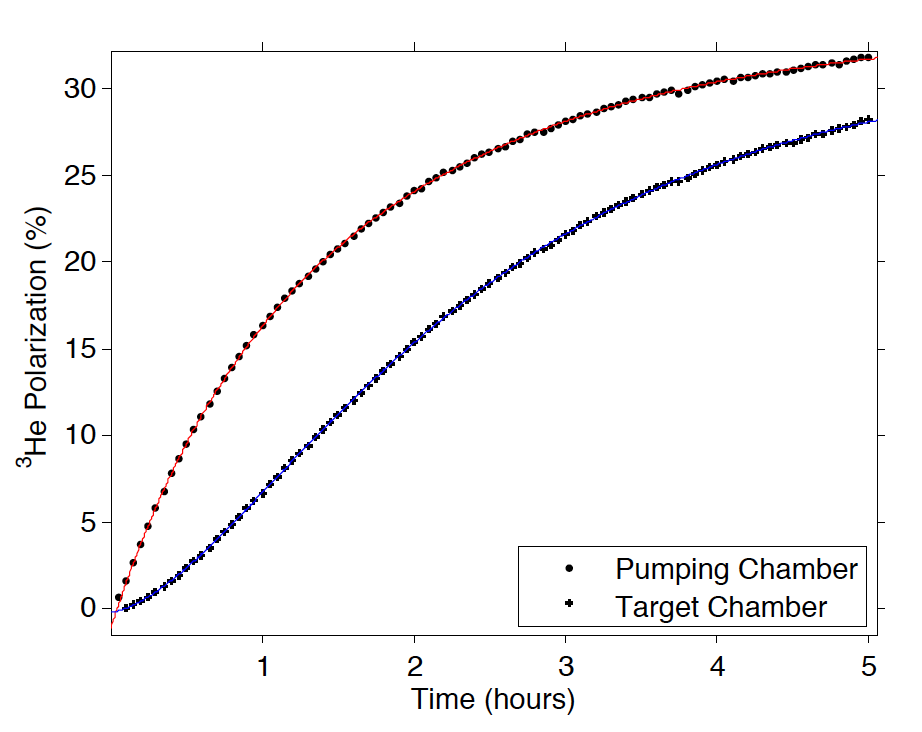
\includegraphics{BradySpinup.png}}
	\caption{{$^{3}$He polarization as a function of time for both the pumping chamber and the target chamber. The top curve is the pumping chamber and the bottom curve is the target chamber. Data was taken at a fast pace so there would be enough points to demonstrate the initial behavior. }}
	\label{BradySpinup}
\end{figure}

\begin{subequations}\label{InitialSpinup}
	\begin{gather}
	P_{pc}(t)=\gamma_{se}P_{A}t-\frac{1}{2}\gamma_{se}P_{A}(\gamma_{se}+\Gamma_{pc}+d_{pc})t^{2}\\
	P_{tc}(t)=\frac{1}{2}\gamma_{se}P_{A}d_{tc}t^{2}
	\end{gather}
\end{subequations}
where $\gamma_{se}$ is the spin-exchange rate in the pumping chamber and $P_{A}$ is the alkali polarization. The dominant term in $P_{pc}(t)$ is the linear term while the shape of $P_{tc}(t)$ is quadratic. 

The slope of the linear shape of initial spinup of the pumping chamber gives access to the product $P_{A}\gamma_{se}$ and fitting the initial spinup of the target chamber to a quadratic function provides the product $\gamma_{se}P_{A}d_{tc}$. The alkali polarization $P_{A}$ can be measured with a technique we refer to here as Faraday rotation, we then gain knowledge of the spin-exchange rate $\gamma_{se}$ and the diffusion rate $d_{tc}$. The slope of the polarization buildup in the pumping chamber is often written as $m_{pc}=P_{A}\gamma_{se}$. 

The spin relaxation rate is also of great importance for characterizing target cells. The relaxation rates in the pumping chamber and the target chamber are different due to geometric and other properties. The cell-average relaxation rate can then be written as

\begin{equation}
\langle \Gamma \rangle=f_{pc}\Gamma_{pc}+f_{tc}\Gamma_{tc}
\end{equation}
where $f_{pc}$ ($f_{tc}$) is the fraction of atoms in PC (TC); $\Gamma_{pc}$ ($\Gamma_{tc}$) is the average relaxation rate in PC (TC). When the cell is being optically pumped, the pumping chamber is heated with hot air to create alkali vapor while the target chamber remains at the room temperature. Difference in temperature further complicates differences in relaxation rates between the two chambers. However, when trying to measure the life time (the inverse of the relaxation rate) of the cell, we typically keep the entire cell at room temperature and perform a ``spindown" measurement. 

During a spindown, the cell starts with some polarization (normally as high as possible so we can obtain a more complete curve), and relaxes on its own while we take AFP measurements at a certain rate. Typically, the interval between measurements is anywhere between 30 mins and 2 hrs, depending on the lifetime of the cell. The rule of thumb is to take AFP frequently enough so the spindown curve has sufficient data points while not too often so the polarization relaxes too fast due to AFP losses. Ideally, the $^{3}$He polarization relaxation can be described by

\begin{equation}\label{Spindown}
P(t)=P_{0}e^{-t/\tau_{true}}
\end{equation}
The true lifetime $\tau_{true}$ of the cell without relaxation due to AFP loss can be measured with two methods: the first is to take 5 AFP measurements consecutively with very short interval (normally around 3 minutes), the second is to perform several spindown measurements, each with a different interval. 

In the first method, because the lifetime of the cell is much longer than 3 minutes, we can safely attribute all losses to AFP measurements and extract the loss due to a single AFP $loss_{afp}$. The data values can then be corrected with the equation

\begin{equation}
S_{i}^{corrected}=S_{i}^{raw}/(1-loss_{afp})^{i-1}
\end{equation}
where $S_{i}^{corrected}$ is the corrected signal, $S_{i}^{raw}$ is the raw signal, i represents it is the $i$th measurement in the spindown, $loss_{afp}$ is the loss due to a single measurement. Fitting the corrected values to Eq.~\ref{Spindown} gives the true lifetime $\tau_{true}$.

A simple example for the second method would be to perform one spindown with one-hour interval and another spindown with two-hour interval, the relaxation rates in these two spindowns are

\begin{subequations}
	\begin{equation}
	\frac{1}{\tau_{1hr}}=\frac{1}{\tau_{true}}+\Gamma_{AFP\_1hr}
	\end{equation}
	\begin{equation}
	\frac{1}{\tau_{2hr}}=\frac{1}{\tau_{true}}+\Gamma_{AFP\_2hr}
	\end{equation}
	\begin{equation}
	\Gamma_{AFP\_1hr}=2\times \Gamma_{AFP\_2hr}
	\end{equation}
\end{subequations}
where $\tau_{1hr}$ and $\tau_{2hr}$ are the lifetimes measured with taking AFP every 1 hour and every 2 hours, $\tau_{true}$ is the true lifetime of the cell without interference from measurements, $\Gamma_{AFP\_1hr}$ ($\Gamma_{AFP\_2hr}$)is the relaxation rate due to taking measurements every 1hr (2hr). We can then solve for $\tau_{true}$.

\section{The K-$^{3}$He Spin-Exchange Rate Constant}

As mentioned in the initial spinup section, the polarization in the pumping chamber at the beginning of the accumulation process, if started in the completely unpolarized state, can be described by 

\begin{equation}
P_{pc} = \gamma_{se}\langle P_{A}\rangle (t-t_{0})+b(t-t_{0})^{2} = m_{pc}t + bt^{2} + c
\end{equation}
where m$_{pc}$ is the slope of the linear term. Typically, in the first 20 to 30 minutes, the spinup behaves so linearly that the effect of quadratic term is negligible.

During these initial spinups, an AFP measurement was taken every 3 minutes, and the AFP losses were carefully accounted for when calculating m$_{pc}$. The $^{3}$He spins were flipped to the opposite direction during every AFP measurement for a short period of time while still receiving polarization in the original direction. Care was taken to account for the time during which spins were ``anti-aligned". We refer to the the slope collected from initial spinups as m$_{pc}^{s}$, to differentiate it from the same quantity measured with the Faraday rotation technique. I will briefly introduce Faraday rotation, the details of which were described thoroughly by Dolph.~\cite{PeterThesis}.

The Faraday rotation technique, as the name implies, is the observation of Faraday rotation using a linearly polarized probe laser. Faraday rotation refers to the change in the orientation of the polarization axis when linearly polarized light passes through a polarized alkali vapor. It is sufficient to consider only the alkali-metal atom's D$_{1}$ and D$_{2}$ lines for our cases. The Faraday rotation angle $\phi_{r}$ is given by:

\begin{equation}\label{rotation_angle}
\phi_r=-\left(\frac{e^2}{12mc\epsilon_0}\right)P[K]l\omega([f_1^{Rb} - f_2^{Rb}]/D + [f_1^K-f_2^K])
\end{equation}
where r$_{e}$ is the classical electron radius, c is the speed of light in vacuum, l is the path length through the vapor, D is the ratio of the K to Rb vapor number densities and $f_1$, $f_2$ are given by
\begin{subequations}\label{fs}
	\begin{gather}
	f_1 = \frac{1}{\omega_{D2}}\frac{\Delta_{D2}}{\Delta_{D2}^2+\frac{\gamma_{D2}^2}{4}}\\
	f_2 = \frac{1}{\omega_{D1}}\frac{\Delta_{D1}}{\Delta_{D1}^2+\frac{\gamma_{D1}^2}{4}}
	\end{gather}
\end{subequations}

During a Faraday rotation measurement, $\phi_{r}$ was measured at several probe wavelengths and fit to the Eq.~\ref{rotation_angle}. We were able to obtain the quantities $P_{A}[Rb]l$ and D from the fit. However, in order ot extract [Rb], it is necessary to measure the path length l and P$_{A}$. Alkali polarization was measured by measuring the Faraday rotation angle while inducing Zeeman transitions. It is worth noting this only gave line-averaged polarization as only information on the path of the probe laser was collected. The volume-averaged alkali polarization can be obtained by applying small corrections from our simulation.

With knowledge of alkali densities, the spin-exchange rate is:

\begin{equation}\label{gammasefr}
\gamma_{se}=k_{se}^{Rb}[Rb]+k_{se}^{K}[K]
\end{equation}
where $k_{se}^{Rb}(k_{se}^{K})$ is the spin-exchange rate constant between $^{3}$He and Rb (K). The m$_{pc}$ calculated with this manner is referred to as ``m$_{pc}^{F}$", since this quantity was computed with Faraday rotation data.

The values of m$_{pc}^{F}$ and m$_{pc}^{s}$ are expected to be the same if they are measured in the same cell under identical conditions. The spin-exchange rate constants $k_{se}^{Rb}$ and $k_{se}^{K}$ are required to calculate m$_{pc}^{F}$. $k_{se}^{Rb}$ has been measured and reported in literature multiple times. $k_{se}^{K}$ on the other hand, is not as well-known. The value of $k_{se}^{Rb}$ we used was the combined result from Baranga \emph{et al.}~\cite{PhysRevLett.80.2801} and from Chann \emph{et al.}~\cite{PhysRevA.66.032703}:

\begin{equation}
k_{se}^{Rb}=(6.79\pm 0.14)\times 10^{-20}{\rm cm}^{3}/{\rm s}
\end{equation}

The ratio of m$_{pc}^{F}$/m$_{pc}^{s}$ is plotted in Fig.~\ref{m_ratio}. The two measurements with the Rb only cell Sosa are shown with solid circles. To calculate the ratio for the rest of the measurements, a value for $k_{se}^{K}$ is needed. Babcock reported this number to be $(5.5\pm 0.4)\times 10^{-20}{\rm cm}^{3}/{\rm s}$ in his thesis~\cite{BabcockThesis}. However, the resulting ratio was significantly lower than unity in all but one of the 6 measurements, as shown with open diamonds in the figure. We fit our data so the ratio m$_{pc}^{F}$/m$_{pc}^{s}$ is equal to one while treating $k_{se}^{K}$ as a free parameter. The results are shown with solid diamonds. Our fitted $k_{se}^{K}$ value is

\begin{equation}
k_{se}^{K}=(7.46\pm 0.62)\times 10^{-20}{\rm cm}^{3}/{\rm s}
\end{equation}

\begin{figure}[t!]
	\centering
	\resizebox{0.91\textwidth}{!}{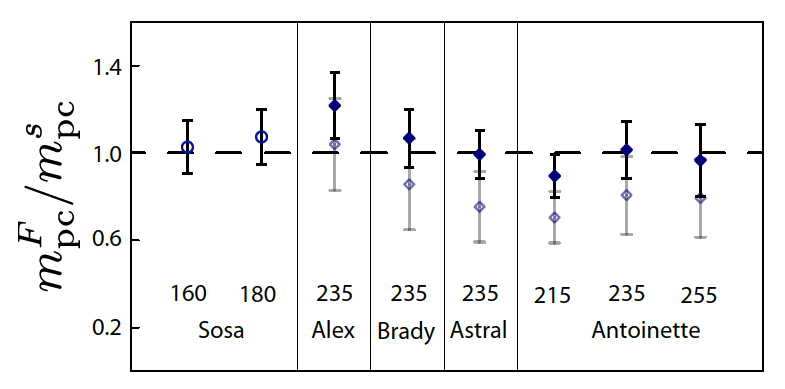
\includegraphics{m_ratio.png}}
	\caption{{Plotted is the ratio m$_{pc}^{F}$/m$_{pc}^{s}$ for eight separate measurements. The numbers above the cell names are the oven set temperatures at which the measurements were made. Difference between open and closed points is discussed in the text.}}
	\label{m_ratio}
\end{figure}

The reason why our result is significantly higher than Babcock's is unclear. One possibility may be temperature dependence as the temperatures under which our measurements were made were higher than that of Babcock's. We decided to use our own result of $k_{se}^{K}$ to measure the X factor because it was measured under similar operating conditions to our other measurements, and our own result improves the internal consistency of our data.

\section{The X Factor}

Prior to the introduction of the X factor, it was not understood why $^{3}$He polarization would not approach unity with sufficiently high alkali-vapor densities and laser power such that $P_{A}$ was nearly 100\% and $\gamma_{se} \gg \langle \Gamma \rangle$. However, the $^{3}$He polarization during our studies had shown differently as also shown by Babcock\emph{et al.}. The fact that it was never close to 100\% even with high laser power and alkali densities could be explained by the X factor.

As mentioned earlier, Babcock~\emph{et al.} reported a previously unrecognized spin relaxation mechanism in his paper~\cite{PhysRevLett.96.083003}. This mechanism appears to be roughly proportional to the spin-exchange rate $\gamma_{se}$, so it cannot be overcome by increasing the alkali density or laser power. The maximal achievable $^{3}$He polarization can be expressed as

\begin{equation}
\lim_{\gamma_{se}\to\infty}=\lim_{\gamma_{se}\to\infty}\frac{\langle P_{A}\rangle\langle \gamma_{se}\rangle}{\langle\gamma_{se}\rangle(1+X)+\langle\Gamma\rangle}=\frac{P_{A}}{1+X}
\end{equation}

The combination of alkali-hybrid and narrowband laser has made it much easier to achieve higher spin-exchange rates $\gamma_{se}$. Thus the X factor is playing an increasingly significant role in limiting the equilibrium $^{3}$He polarization, which makes it an important subject for study.

Unlike many other properties of the cell that can be measured directly, the X factor is a derived quantity. While characterizing our target cells, we collected enough data to determine the X factor in several different ways. We were able to compare these values and combine them into weighted averages. We also looked at possible temperature dependence using X values obtained at different temperatures. The data used are presented in Table~\ref{table:CellTable}.

\begin{table*}\tiny
	\captionsetup{font=scriptsize}
	\begin{center}
		\def\arraystretch{0.75}
		\setlength\tabcolsep{0.5pt}
		\begin{tabular}{|c|c|ccc|ccc|ccccc|cc|c|}
			\hline
			\multirow{2}{*}{\begin{sideways}{EXP}\end{sideways}}&\multirow{2}{*}{Cell} & \multirow{2}{*}{Lasers} & $I_0$ & T$_\mathrm{pc}^\mathrm{set}$ & \multirow{2}{*}{$P_\mathrm{He}^\infty$} & $\Gamma_\mathrm{s}^{-1}$ & $\langle\Gamma\rangle^{-1}$ & \multirow{2}{*}{$\langle P^\mathrm{A} \rangle$} & \multirow{2}{*}{$P_\mathrm{line}^\mathrm{A}$} & \multirow{2}{*}{$D_\mathrm{fr}$} & \multirow{2}{*}{$D_\mathrm{pb}$} & [Rb]$_\mathrm{fr}$ & $\Delta$T$_\mathrm{Rb}$ & $\Delta$T$_\mathrm{He}$ & \multirow{2}{*}{X}\\
			&& & W/cm$^2$ & $^\circ$C & & hrs & hrs & & & & & $10^{14}$/cm$^3$ & $^\circ$C & $^\circ$C &\\
			\hline
			\hline
			\multirow{5}{*}{\begin{sideways}saGDH\end{sideways}} & Proteus & 3B & 3.8 & 180 & 0.46 & 27 & 74 & - & - & 0 & 0 & - & - & - & -\\
			\cline{2-16}
			& Priapus & 3B & 3.8 & 180 & 0.44 & 21 & 56 & - & - & 0 & 0 & - & - & - & -\\
			\cline{2-16}
			& Penelope & 3B & 3.8 & 180 & 0.39 & 18 & 46 & - & - & 0 & 0 & - & - & - & -\\
			\cline{2-16}
			& Powell & 3B & 3.8 & 180 & 0.38 & 13 & 25 & - & - & 0 & 0 & - & - & - & -\\
			\cline{2-16}
			& Prasch & 3B & 3.8 & 180 & 0.33 & 13 & 33 & - & - & 0 & 0 & - & - & - & -\\
			\hline
			\hline
			\multirow{20}{*}{\begin{sideways}GEN\end{sideways}} & \multirow{2}{*}{Al} & 2.5B & 3.2 & 235 & 0.53(03) & 7.86(05) & 27.42(1.37) & - & - & - & 4.53(25) & - & - & - & - \\
			& & 5B & 6.1 & 235 & 0.54(03) & 6.73(18) & 27.42(1.37) & - & - & - & 4.53(25) & - & - & - & - \\
			\cline{2-16}
			& \multirow{2}{*}{Barbara} & 2.5B & 1.6 & 235 & 0.37(02) & 5.5(08) & 42.95(2.15) & - & - & - & 4.80(25) & - & - & - & - \\
			& & 5B & 3.1 & 235 & 0.57(03) & 4.76(63) & 42.95(2.15) & - & - & - & 4.80(25) & - & - & - & - \\
			\cline{2-16}
			& Gloria & 3B & 1.7 & 235 & 0.60(03) & 6.13(04) & 38.29(1.91) & - & - & - & 7.20(40) & - & - & - & - \\
			\cline{2-16}
			& \multirow{2}{*}{Anna} & 1B & 0.6 & 235 & 0.33(02) & 5.60(34) & 11.38(57) & - & - & - & 9.64(57) & - & - & - & - \\
			& & 1.5B & 1.0 & 235 & 0.39(02) & 5.37(08) & 11.38(57) & - & - & - & 9.64(57) & - & - & - & - \\
			\cline{2-16}
			& \multirow{2}{*}{Dexter} & 1.5B & 1.5 & 235 & 0.47(02) & 7.58(17) & 18.45(92) & - & - & - & - & - & - & - & - \\
			& & 5B & 6.1 & 235 & 0.49(02) & 6.63(12) & 18.45(92) & - & - & - & - & - & - & - & - \\
			\cline{2-16}
			& Edna & 3B & 2.4 & 235 & 0.56(03) & 5.71(02) & 27.42(1.37) & - & - & - & 3.63(20) & - & - & - & - \\
			\cline{2-16}
			& \multirow{2}{*}{Dolly} & 3B & 1.0 & 235 & 0.43(02) & 6.16(03) & 35.24(1.76) & - & - & - & 20(1.3) & - & - & - & - \\
			& & 1N1B & 1.4 & 235 & 0.62(03) & 5.79(07) & 35.24(1.76) & - & - & - & 20(1.3) & - & - & 17(10) & - \\
			\cline{2-16}
			& \multirow{3}{*}{Simone} & 2N1B & 3.8 & 215 & 0.31(01) & 14.08(06) & 22.87(1.14) & 0.947(020)  & 0.91(05) & 10.66(54) & 8.89(45) & 0.20(02) & -7(3) & - & -0.04(12)$^\star$ \\
			& & 2N1B & 3.8 & 240 & 0.48(02) & 6.89(20) & 22.87(1.14) & - & - & - & 9.76(49) & - & - & - & - \\
			& & 2N1B & 3.8 & 255 & 0.58(02) & 6.45(10) & 22.98(1.14) & 0.929(023) & 0.92(05) & 12.48(83) & 10.3(52) & 0.90(09) & -4(5) & - & 0.11(06)$^\star$ \\
			\cline{2-16}
			& \multirow{5}{*}{Sosa} & 2N1B & 1.9 & 160 & 0.57(02) & 16.69(09) & 73.68(3.68) & 0.966(020) & 1.00(03) & 0 & 0 & 1.97(13) & 4(1) & 30(7) & 0.24(06)$^\dagger$ \\
			&  & 2N1B & 1.9 & 170 & 0.61(03) & 11.67(04) & 73.68(3.68) & 0.964(020) & 0.98(03) & 0 & 0 & 3.00(33) & 3(3) & 38(14) & 0.27(06)$^\star$ \\
			&  & 2N1B & 1.9 & 180 & 0.55(02) & 8.79(09) & 73.68(3.68) & 0.954(022) & 0.97(03) & 0 & 0 & 4.30(27) & 1(2) & 47(7) & 0.43(06)$^\dagger$ \\
			&  & 2N1B & 1.9 & 190 & 0.40(02) & 6.39(22) & 73.68(3.68) & 0.854(075) & 0.82(03) & 0 & 0 & 5.69(63) & -2(3) & 48(20) & 0.58(12)$^\star$ \\
			&  & 2N1B & 1.9 & 200 & 0.26(01) & 5.04(17) & 73.68(3.68) & - & - & 0 & 0 & - & - & 43(18) & - \\
			%& 2C1F & 1.9 & 160 & 0.57(03) & 16.7(09) & 55.7(1.8) & 1.00(03) & 0 & 0 & -\\
			% & 2C1F & 1.9 & 170 & 0.61(03) & 11.7(03) & 55.5(2.0) & 0.98(03) & 0 & 0 & -\\
			% & 2C1F & 1.9 & 180 & 0.55(03) & 8.79(09) & 55.2(2.2) & 0.97(03) & 0 & 0 & - \\
			% & 2C1F & 1.9 & 190 & 0.40(02) & 6.39(22) & 55.1(2.3) & - & 0 & 0 & -\\
			% & 2C1F & 1.9 & 200 & 0.26(01) & 5.40(17) & 55.4(2.1) & 0.83(17) & 0 & 0 & -\\
			\hline
			\hline
			\multirow{12}{*}{\begin{sideways}Transversity\end{sideways}} & Boris & 3B & 1.8 & 235 & 0.42(02) & 6.25(04) & 23.74(1.19) & 0.871(050) & 0.79(07) & 1.96(18) & 2.45(23) & 2.19(34) & -8(7) & - & 0.26(10)$^\star$ \\
			\cline{2-16}
			& \multirow{2}{*}{Samantha} & 3B & 1.8 & 235 & 0.50(02) & 6.30(13) & 36.51(1.83) & - & - & - & 4.34(23) & - & - & - & -\\
			& & 3N & 2.6 & 235 & 0.68(03) & 4.62(03) & 22.13(1.11) & 0.956(020) & 0.99(03) & 4.37(10) & 4.34(23) & 1.80(10) & 7(2) & 21(10) & 0.12(05)$^\star$\\
			\cline{2-16}
			& Alex & 2N1B & 2.6 & 235 & 0.59(03) & 4.81(02) & 32.96(1.65) & 0.942(042) & 0.99(03) & 1.37(08) & 1.19(07) & 4.08(36) & 0(4) & 42(10) & 0.34(06)$^\dagger$ \\
			\cline{2-16}
			& Moss & 1N1B & 1.8 & 235 & 0.62(03) & 5.35(04) & 33.00(1.65) & - & 0.95(09) & - & 2.40(13) & - & - & 29(8) & -\\
			\cline{2-16}
			& Tigger & 1N1B & 1.8 & 235 & 0.51(02) & 4.89(05) & 12.62(63) & - & 0.95(09) & - & - & - & - & 23(9) & -\\
			\cline{2-16}
			& Astral & 2N1B & 2.6 & 235 & 0.69(03) & 6.57(12) & 48.90(2.45) & 0.954(020) & 0.99(03) & 7.09(55) & 6.21(56) & 0.97(09) & 3(5) & 25(4) & 0.17(05)$^\dagger$\\
			\cline{2-16}
			& Stephanie & 3N & 2.6 & 235 & 0.63(03) & 4.55(09) & 48.35(2.42) & 0.929(114) & 0.99(03) & 1.39(11) & 1.50(10) & 5.08(58) & 7(5) & 54(6) & 0.31(08)$^\star$\\
			\cline{2-16}
			& \multirow{3}{*}{Brady} & 1N & 0.9 & 235 & 0.62(03) & 4.82(1.08) & 33.50(1.68) & - & 0.95(03) & - & 2.36(24) & -  & - & 14(9) & -\\
			& & 2N & 1.8 & 235 & 0.68(03) & 5.52(70) & 33.50(1.68) & - & 0.99(03) & - & 2.36(24) & - & - & 25(8) & -\\
			& & 3N & 2.6 & 235 & 0.70(03) & 5.30(01) & 33.50(1.68) & 0.956(021) & 0.99(03) & 2.60(20) & 2.36(24) & 2.86(30) & 6(5) & 39(9) & 0.14(05)$^\dagger$\\
			\cline{2-16}
			& Maureen & 3N & 2.6 & 235 & 0.66(03) & 5.42(12) & 29.21(1.46) & - & 0.97(09) & - & 4.42(55) & - & - & 32(12) & -\\
			\cline{2-16}
			&Antoinette & 3N & 1.7 & 215 & 0.49(02) & 6.63(37) & 20.93(1.05) & 0.958(020) & 0.99(03) & 2.85(13) & - & 0.96(07) & 0(3) & 16(8) & 0.28(08)$^\dagger$\\
			& & 3N & 1.7 & 235 & 0.61(03) & 4.18(10) & 20.93(1.05) & 0.936(043) & 0.99(03) & 3.32(27) & - & 1.83(20) & 0(5) & 20(10) & 0.24(07)$^\dagger$\\
			& & 3N & 1.7 & 255 & 0.41(02) & 2.66(11) & 20.93(1.05) & 0.776(099) & 0.93(10) & 3.57(23) & - & 2.88(39) & -5(6) & 33(9) & 0.55(13)$^\dagger$\\
			\hline
		\end{tabular}
		\caption
		{Cell Performance for three sets of experiments: saGDH (top), GEN (middle), and Transversity \& $d_2^n$ (bottom).  Within each experiment grouping, data is grouped by type of laser used (B = Broadband, N = Narrowband). $I_0$ is the nominal incident laser intensity at the center of the pumping chamber. $T_{pc}^{set}$ is the oven set temperature. $P_{pc}^\infty$ is the equilibrium polarization in the pumping chamber and $\Gamma_s$ is the slow time constant extracted from the five parameter fit to the polarization build up curve. $\Gamma_c$ is the cell-averaged room temperature spin relaxation rate. $\langle P_A\rangle/P_A^l$ is the volume averaged to line averaged alkali polarizaiton ratio determined from the optical pumping simulation. $P_A^l$ is the measured line averaged alkali polarization. $D_{fr} \& D_{pb}$ are the K to Rb density ratios determined from Faraday rotation and pressure broadening measurements. [Rb]$_{fr}$ is the Rb number density measured from Faraday rotation. $\Delta T_{He}$ is the temperature of Rb inferred from the number density relative to the oven set temperature. $\Delta T_{He}$ is the temperature of $^3$He inferred from temperature tests relative to the oven set temperature. X is the best combined value for the X-factor. $^\star$ indicates X was measured using only spinup, alkali polarization, and Faraday rotation data. $^\dagger$ indicates X was also measured using the early-time behavior of the spinup.}
		\label{table:CellTable}
	\end{center}
\end{table*}


We calculated the X factors in several different ways, all of which required knowledge of the cell-averaged spin relaxation rate $\langle \Gamma\rangle$ at operating temperatures. However, the spindown measurements we performed only gave us the spin relaxation rate $\langle \Gamma\rangle_{c}$ at room temperature. We made the assumption that the difference between $\langle \Gamma\rangle$ and $\langle \Gamma\rangle_{c}$ is purely due to the change of cell-averaged $^{3}$He-$^{3}$He dipolar spin relaxation rate, and the relaxation rate due to collisions with the walls is the same for the two chambers and does not change at different temperature. The correction to the relaxation rate is given by

\begin{equation}
\langle \Gamma\rangle=\langle \Gamma\rangle_{c}-[n_{0}-f_{pc}n_{pc}/f^{d}(t_{pc})- f_{tc}n_{tc}/f^{d}(t_{tc})]/\tau^{d}
\end{equation}
where n$_{0}$ is the $^{3}$He fill density, n$_{pc(tc)}$ is the $^{3}$He density in the pumping (target) chamber, f$_{pc(tc)}$ is the fraction of $^{3}$He atoms in the pumping (target) chamber, $t_{pc}=T_{pc}/(296.15 K)$, $t_{tc}=(313.15 K)/(296.15 K)$, $\tau^{d}=744 hrs\cdot amg$~\cite{PhysRevA.48.4411}, $f^{d}(t)$ is a function that parameterizes the temperature dependence of the dipolar relaxation~\cite{JaideepThesis}. $\langle \Gamma\rangle$ is typically only a few percent less than $\langle \Gamma\rangle_{c}$ for us. In addition, whenever the quantity $(\Gamma_{s}-\langle \Gamma\rangle)$ is used, a small correction to account for the AFP losses is added.

Our methods of extracting X require using some form of the equation

\begin{equation}\label{gammase}
\langle \gamma_{se}\rangle=\frac{\Gamma_{s}-\langle \Gamma\rangle+\delta\Gamma}{1+X}
\end{equation}

One method Babcock used and we applied on a small number of cells is called ``hot relaxation method"~\cite{PhysRevLett.96.083003}. We plot $\langle \gamma_{se}\rangle$ as a function of $\Gamma_s - \langle\Gamma\rangle + \delta\Gamma$, the slope of a linear fit to the data is expected to be 1/(1+X). Three such fits are shown in Fig.~\ref{hotrelaxation}, all of which were constrained to go through the origin. Two of the three X values were significantly different than zero. The X factor of Simone is too close to zero when the error is taken into account for us to make a strong statement.

The small correction $\delta\Gamma$ came into play because of the double-chambered design. It can be approximated by

\begin{equation}
\delta\Gamma\approx f_{pc}f_{tc}(d_{pc}+d_{tc})u^2 + higher~order~terms
\end{equation}
where $d_{pc(tc)}$ is the probability per unit time that a $^3$He atom will exit the pumping (target) chamber. The quantity u is 

\begin{equation}\label{u}
u=\frac{\gamma_{se}(1+X)+\Gamma_{pc}-\Gamma_{tc}}{d_{pc}+d_{tc}}
\end{equation}
where $\Gamma_{pc(tc)}$ is the spin relaxation rate in the pumping (target) chamber. What makes the determination of X tricky is that we need to know its value before we can calculate u which is a prerequisite for X. However, because $\delta\Gamma$ is such a small correction typically being 10\% of less of the size of $\Gamma_s$, we solve this problem in an iterative manner. X is initially assumed to be 0 and plugged into Eq.~\ref{u}, which in the end lead to a different value of X that is closer to its real value. After iterating this process a few times, X quickly converges to a stable value.

\begin{figure}[t!]
	\centering
	\resizebox{0.91\textwidth}{!}{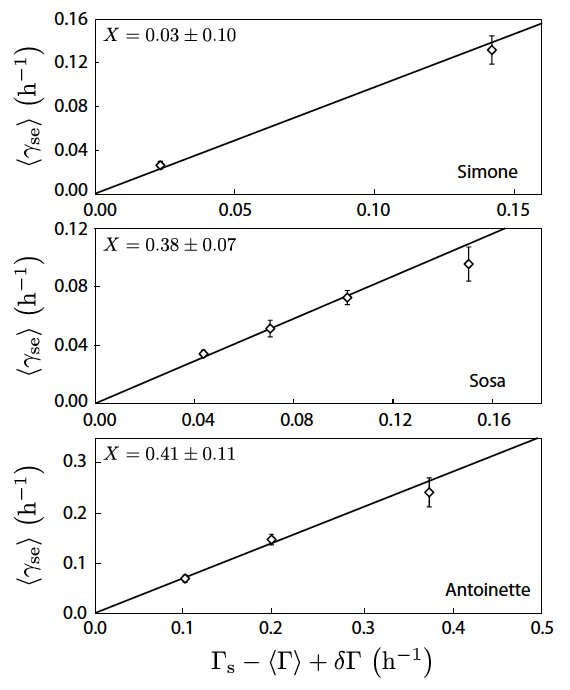
\includegraphics{hotrelaxation.png}}
	\caption{{The cell-averaged spin-exchange rate $\langle\gamma_{se}\rangle$ is calculated using data from Faraday rotation and the spin-exchange constants $k_{se}^{Rb}$ and $k_{se}^{K}$. The three linear fits shown here are constrained to go through zero. The errors quoted in values of X factor include the uncertainty in our determination of $k_{se}^{K}$.}}
	\label{hotrelaxation}
\end{figure}

However, the hot relaxation method assumes the temperature dependence of the X factor is identical to the temperature dependence of $\gamma_{se}$ by combining data taken at different temperature into one value of X. It is also time consuming to perform the measurements shown in Fig.~\ref{hotrelaxation}. For these two reasons, the hot relaxation method was only applied to a small number of cells. 

In order to measure the X factor at a single temperature and explore its possible temperature dependence, we used 4 four other methods to determine the value of X factor. All but the second method described below are based on the ``polarization method" from Ref.~\cite{PhysRevLett.96.083003}. And the second method is basically a single point measurement of the hot relaxation method described above.

We label the results from the four single-temperature methods as $X_1$, $X_2$, $X_3$ and $X_4$ respectively. The most straightforward method requires measurements of $\langle P_A\rangle$, $P_{pc}^\infty$ and $\Gamma_s$. The equilibrium $^3$He polarization can be rewritten as

\begin{equation}\label{pinfty}
P_{pc}^\infty=\frac{\langle P_A\rangle\langle\gamma_{se}\rangle}{\Gamma_s+\delta\Gamma-\delta\Gamma'}
\end{equation}
where $\delta\Gamma'=f_{tc}\Gamma_{tc}^2/(\Gamma_{tc}+d_{tc}).$ Substituting Eq.~\ref{gammase} into Eq.~\ref{pinfty}, we find

\begin{equation}
X_1=\frac{\langle P_A\rangle}{P_{pc}^\infty}\left(\frac{\Gamma_s-\langle\Gamma\rangle+\delta\Gamma}{\Gamma_s+\delta\Gamma-\delta\Gamma'}\right)-1
\end{equation}

Just as what we did for the hot relaxation method, here $\delta\Gamma$ is calculated in the same iterative manner. X is first taken as 0 and the iteration continued until X converged to a stable value.

For the second method, we first solve Eq.~\ref{gammase} for X:

\begin{equation}\label{x23}
X=\frac{\Gamma_s-\langle\Gamma\rangle+\delta\Gamma}{\langle\gamma_{se}\rangle}-1
\end{equation}
then we substitute Eq.~\ref{gammasefr} into the equation above:

\begin{equation}
X_2=\frac{\Gamma_s-\langle\Gamma\rangle+\delta\Gamma}{f_{pc}k_{se}^{Rb}[Rb](1+D')}-1
\end{equation}
where 
\begin{equation}
D'=Dk_{se}^K/k_{se}^{Rb}
\end{equation}

Again $\delta\Gamma$ is calculated iteratively. We chose to use our value of $k_{se}^{K}$ for better consistency with the rest of our data.

The third method is very similar to the second, but we determine $\langle\gamma_{se}\rangle$ with data from initial spinups:

\begin{equation}
\langle\gamma_{se}\rangle=f_{pc}m_{pc}^{s}/\langle P_A\rangle
\end{equation}

Substitute the above equation into Eq.~\ref{x23}, we get

\begin{equation}
X_3=\langle P_A\rangle\frac{\Gamma_s-\langle\Gamma\rangle+\delta\Gamma}{f_{pc}m_{pc}^s}-1
\end{equation}

Note the quantity $k_{se}^K$ used for $X_2$ was obtained by fitting the ratio $m_{pc}^F/m_{pc}^s$ to 1, thus for any hybrid cell, $X_2$ and $X_3$ are highly correlated. However, for pure Rb cell such as Sosa, these two methods are independent.

The difference between the fourth method and the first is that the fourth method treats $\langle\gamma_{se}\rangle$ as a known quantity and expresses $\Gamma_s$ with it using Eq.~\ref{gammase}, while the first method did it in the opposite way. The cell-averaged spin-exchange rate is evaluated with 

\begin{equation}
\langle\gamma_{se}\rangle=f_{pc}m_{pc}^s/\langle P_A\rangle
\end{equation}

Thus $X_4$ is

\begin{equation}
X_4=\frac{P_A}{P_{pc}^\infty}-\frac{\langle P_A\rangle(\langle\Gamma\rangle-\delta\Gamma')}{f_{pc}m_{pc}^s}-1
\end{equation}

\begin{table*}
	\scriptsize
	\captionsetup{font=small}
	\begin{center}
		\def\arraystretch{0.75}
		\setlength\tabcolsep{1pt}
		\begin{tabular}{|c|c|cccc|c|}
			\hline
			Cell & T($^\circ$C) & $X_1$ & $X_2$ & $X_3$ & $X_4$ & $X_{12}/X_{1234}$\\ 
			\multirow{2}{*}{Simone} & 215 & -0.02(12) & -0.10(14) & - & - & -0.04(12) \\
			& 255 & 0.13(08) & 0.08(09) & - & - & 0.11(06) \\
			\hline
			\multirow{4}{*}{Sosa} & 160 & 0.22(07) & 0.28(09) & 0.32(15) & 0.18(09) & 0.24(06)$^\dagger$ \\
			& 170 & 0.24(07) & 0.37(15) & - & - & 0.27(06)\\
			& 180 & 0.45(08) & 0.40(09) & 0.50(17) & 0.45(09) & 0.43(06)$^\dagger$ \\
			& 190 & 0.59(16) & 0.57(17) & - & - & 0.58(12) \\
			\hline
			\hline
			Boris & 235 & 0.21(14) & 0.31(14) & - & - & 0.26(10)\\
			\hline
			Sam. & 235 & 0.08(06) & 0.22(09) & - & - & 0.12(05) \\
			\hline
			Alex & 235 & 0.34(09) & 0.35(09) & 0.63(20) & 0.29(10) & 0.34(06)$^\dagger$\\
			\hline
			Astral & 235 & 0.15(07) & 0.22(10) & 0.20(14) & 0.14(07) & 0.17(05)$^\dagger$\\
			\hline
			Steph. & 235 & 0.31(17) & 0.31(10) & - & - & 0.31(08)\\
			\hline
			Brady & 235 & 0.13(07) & 0.15(09) & 0.23(14) & 0.11(07) & 0.14(05)$^\dagger$\\
			\hline
			\multirow{3}{*}{Antoinette} & 215 & 0.27(09) & 0.44(17) & 0.30(19) & 0.25(11) & 0.28(08)$^\dagger$\\
			& 235 & 0.20(09) & 0.34(12) & 0.36(17) & 0.15(09) & 0.24(07)$^\dagger$\\
			& 255 & 0.55(26) & 0.54(16) & 0.50(30) & 0.56(26) & 0.55(13)$^\dagger$\\
			\hline
		\end{tabular}
		\caption
		{Shown are the values of the X factor at the indicated over set temperatures. The last column is a weighted average of results from either the first two methods or all four methods. A $^\dagger$ indicates combined values computed with all 4 methods.}
		\label{Xtable}
	\end{center}
\end{table*}

The computed X factors are shown in Table~\ref{Xtable}. The different values of X are quite consistent with each other. It is worth noting that even though $X_1$ is completely independent of $m_{pc}$ and $k_{se}^K$, it is still quite consistent with the rest of the X values. The last column in the table is a weighted average of either $X_1$ and $X_2$ ($X_{12}$) or all four X values ($X_{1234}$). 

To the best of our knowledge, there has not been a dedicated study of the X factors and the their temperature dependence, with a large number of cells using measurements of the alkali polarization since the original work of Babcock's~\emph{et al.} original work~\cite{PhysRevLett.96.083003}. Our results thus represents independent evidence of the existence of a non-zero X factor. According to our study, the X factor limits $^3$He polarization to 62-88\% for the range of temperature we operate within.

Since we have evaluated X at multiple temperatures for Simone, Sosa and Antoinette, we can explore the temperature dependence of X factor. The combined value of X is plotted against temperature in Fig.~\ref{XvsT} for the three cells. The figure seems to indicate a systematic variation with temperature.

\begin{figure}[t!]
	\centering
	\resizebox{0.91\textwidth}{!}{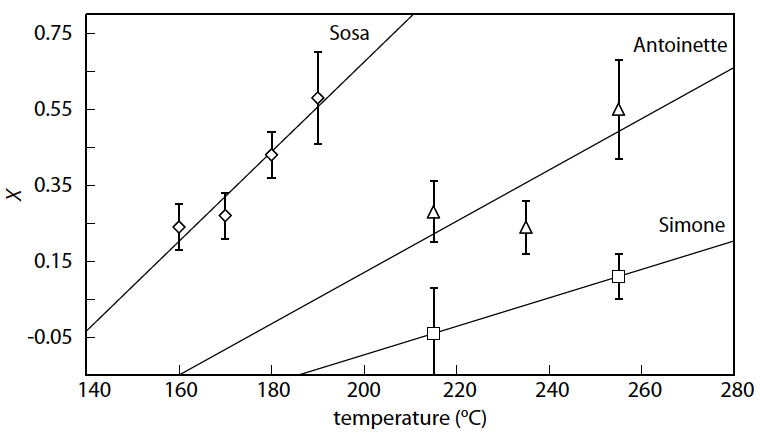
\includegraphics{XvsT.png}}
	\caption{{Shown are the combined values for X factor (either $X_{12}$ or $X_{1234}$ depending on the availability of data) versus temperature for the cell Sosa, Simone and Antoinette.}}
	\label{XvsT}
\end{figure}

If we assume a linear dependence of X with temperature, the fitted slope for Sosa with 4 points is ($0.012\pm0.002)/^\circ C$, which is six-sigma away from zero. The slope for the three points of Antoinette is $(0.007\pm0.005)/^\circ C$, which is slightly above one sigma from zero. Simone has only two points available to us, the second point seems to be right around the edge of the error bar on the first point. Although we cannot make a strong statement, it seems likely that there is a trend here. We do not consider this result conclusive, but it still suggests the existence of temperature dependence of X.

We considered the possibility that the temperature dependence was introduced by our own value of the spin-exchange constant $k_{se}^{K}$. After considering both our value and that from Babcock, we found that the trend exists with both, but our value provides better self consistency. Another possibility is that the temperature dependence of $k_{se}^{K}$ is the source of temperature dependence of X. However, if that is the case, we should be able to observe different behaviors in what the 4 different methods produced. From what is shown by Table~\ref{Xtable}, the different methods produced similar results within errors, thus $k_{se}^K$ is not likely to be the cause of temperature dependence of X.

Another possibility was the temperature dependent contribution from anisotropic spin exchange~\cite{PhysRevA.81.032709}. However, even though calculations from Tscherbul \emph{et al.}~\cite{PhysRevLett.107.023204} indicate the anisotropic spin exchange contribution to the X factor has a temperature dependence, the contribution is very small in our operating temperature range.

We also considered whether other systematic effects could result in such temperature dependence. For example, the distribution of the gas between pumping chamber and target chamber changes at different temperatures. We then concluded that the uncertainties in the gas distribution had only negligible effects on the observed temperature dependence of X. After analyzing our data, we were unable to identify a systematic effect as a plausible explanation, our results suggest further study of X and its temperature dependence may be of great importance.
















